%Введение и постановка задачи 
The mitral valve, also known as the bicuspid valve or left atrioventricular
valve, is a valve with two flaps in the heart, that lies between the left atrium
and the left ventricle. The mitral valve and the tricuspid valve are known
collectively as the atrioventricular valves because they lie between the atria
and the ventricles of the heart.
\begin{figure}[H]
  \centering
  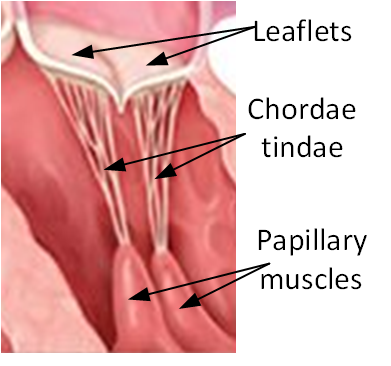
\includegraphics[width=0.4\columnwidth]{./fig/mt.png}
  \caption{Mitral valve structure}
  \label{fig:MT}
\end{figure}
Mitral valve has cyclic working conditions. The valve opens and closes because
of pressure differences, opening when there is greater pressure in the left
atrium than ventricle, and closing when there is greater pressure in the
ventricle than atrium. In abnormal conditions, blood may flow backwards through
the valve (mitral regurgitation) or the mitral valve may be narrowed (mitral
stenosis). Mitral valve prolapse (MVP) is a valvular heart disease characterized
by the displacement of an abnormally thickened mitral valve leaflet into the
left atrium during systole. By other words, it is a condition in which the two
flaps of the mitral valve doesn't close smoothly and evenly, but instead bulge
(prolapse) upward into the left atrium.\cite{Hayek2005a}
\begin{figure}[H]\label{fig:compareMT}
  \centering
  \begin{subfigure}[H]{0.42\columnwidth}\label{fig:normalMT}
    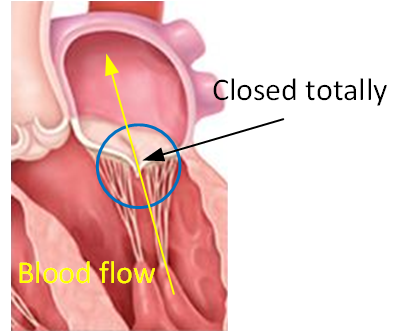
\includegraphics[width=\columnwidth]{./fig/normalMT.png}
    \caption{Normal}
  \end{subfigure}
  \begin{subfigure}[H]{0.4\columnwidth}\label{fig:prolapseMT}
    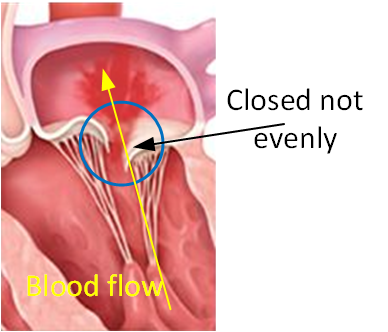
\includegraphics[width=\columnwidth]{./fig/prolapseMT.png}
    \caption{Prolapse}
  \end{subfigure}
  \caption{Prolapse in compare to normal}
\end{figure}
\cm{To solve such disease by surgical way, usually "methd" is used. link for article}
Providing the surgeon with an anatomically and biomechanically accurate
computional model of a particular patient's mitral heart valve could enable
preoperative surgical planning and potentially improve surgical outcome.

There are a large number of different numerical modeling methods. All of them are
derivatives of Finite Element Method(FEM) and Discrete Element Method(DEM).
While general finite-element studies are helpful for the evaluation and
development of MV repair surgery, patient-specific models are required for
individual therapy planning. The patient-specific mass-spring MV model uses a
segmentation of 3D TEE images for the initialization of a mass-spring model of
the closed MV under systolic pressure. An iterative approach is used to adjust
the spring rest-length so that the model can accurately simulate the shape of
the closed MV under systolic pressure. To simulate MV annuloplasty, the model
can then be deformed, according to the annuloplasty ring to be used, to create a
prediction of the shape of the closed MV after surgery.

Based on the properties of the material of biological tissues and review of
existing projects, the most appropriate method is Mass - Spring modeling(MSM).
This method based on ideas of DEM and basic element here is very know in
mechanic simple one dimensional(1D) beam.

Computational complexity of MSM is much less compare to FEM-based methods,
because of less number of equations to integrate on each time step. This
important advantage and physics way have method describes basic element gave to
MSM very wide using in computer games for calculating reality-looks hair or
cloth movement in real time. Modelling by using MSM could be parallel calculated
on each time step.\cite{Rasmusson2008} \cite{Amorim2012}
